% !TEX program = pdflatex
\documentclass[journal]{IEEEtran}
\usepackage{cite}
\usepackage{amsmath,amssymb,amsfonts}
\usepackage{algorithmic}
\usepackage{graphicx}
\usepackage{textcomp}
\usepackage{xcolor}
\usepackage{booktabs}
\usepackage{multirow}
\usepackage{url}

\def\BibTeX{{\rm B\kern-.05em{\sc i\kern-.025em b}\kern-.08em
    T\kern-.1667em\lower.7ex\hbox{E}\kern-.125emX}}

\begin{document}

\title{Physics-Guided Synthetic WiFi CSI Data Generation for Trustworthy Human Activity Recognition: A Sim2Real Approach}

\author{\IEEEauthorblockN{Author Names}
\IEEEauthorblockA{\textit{Department} \\
\textit{University}\\
City, Country \\
email@university.edu}}

\maketitle

\begin{abstract}
WiFi Channel State Information (CSI) based Human Activity Recognition (HAR) promises device-free, privacy-preserving sensing, yet faces two practical impediments: scarcity of labeled data and poor cross-domain generalization. We propose a physics-guided synthetic CSI generation framework and an Enhanced deep model that combines CNN feature extraction, squeeze-and-excitation (SE) channel attention, and temporal attention, coupled with trustworthy evaluation (calibration, reliability). Comprehensive experiments on synthetic robustness (D6), cross-domain adaptation (CDAE: LOSO/LORO), and Sim2Real transfer efficiency (STEA) demonstrate that our approach attains identical 83.0±0.1\% macro F1 across LOSO/LORO and achieves 82.1\% macro F1 using only 20\% labeled real data, narrowing the gap to full supervision (83.3\%) while reducing labeling cost by 80\%. The results support physics-guided synthesis and calibrated inference as practical tools for reliable, sample-efficient CSI HAR.
\end{abstract}

\begin{IEEEkeywords}
WiFi CSI, Human Activity Recognition, Synthetic Data, Sim2Real, Calibration, Cross-Domain Generalization
\end{IEEEkeywords}

\section{Introduction}
WiFi CSI enables device-free HAR via the perturbations human motion induces on multipath wireless channels. Compared with cameras and wearables, CSI is unobtrusive and privacy-preserving; in practice, however, two issues dominate: acquiring labeled data is labor-intensive, and models that excel in one domain often degrade in another. SenseFi~\cite{yang2023sensefi} consolidates supervised baselines and datasets, yet it presumes ample labels and does not directly address Sim2Real deployment.

We revisit CSI HAR through a physics-grounded, evaluation-first lens. Our framework generates synthetic CSI by modeling multipath, human-body interaction, and environmental variability, and trains an Enhanced architecture with SE channel attention and temporal attention to emphasize informative subcarriers and long-range temporal cues. Beyond accuracy, we incorporate trustworthy metrics—Expected Calibration Error (ECE), Brier, Negative Log-Likelihood (NLL)—to quantify reliability. Our study asks: can we obtain robust cross-domain performance and strong label efficiency, with calibrated probabilities suited for safety-critical IoT?

\textbf{Contributions}—(1) a physics-guided generator for flexible, parameterized CSI synthesis; (2) a Sim2Real evaluation covering CDAE and STEA; (3) a sample-efficiency result of 82.1\% macro F1 with 20\% labels (98.6\% of full 83.3\%); (4) trustworthy evaluation with improved calibration; and (5) an Enhanced CNN+SE+temporal attention model achieving LOSO/LORO parity (83.0±0.1\%).

\begin{figure}[t]
\centering
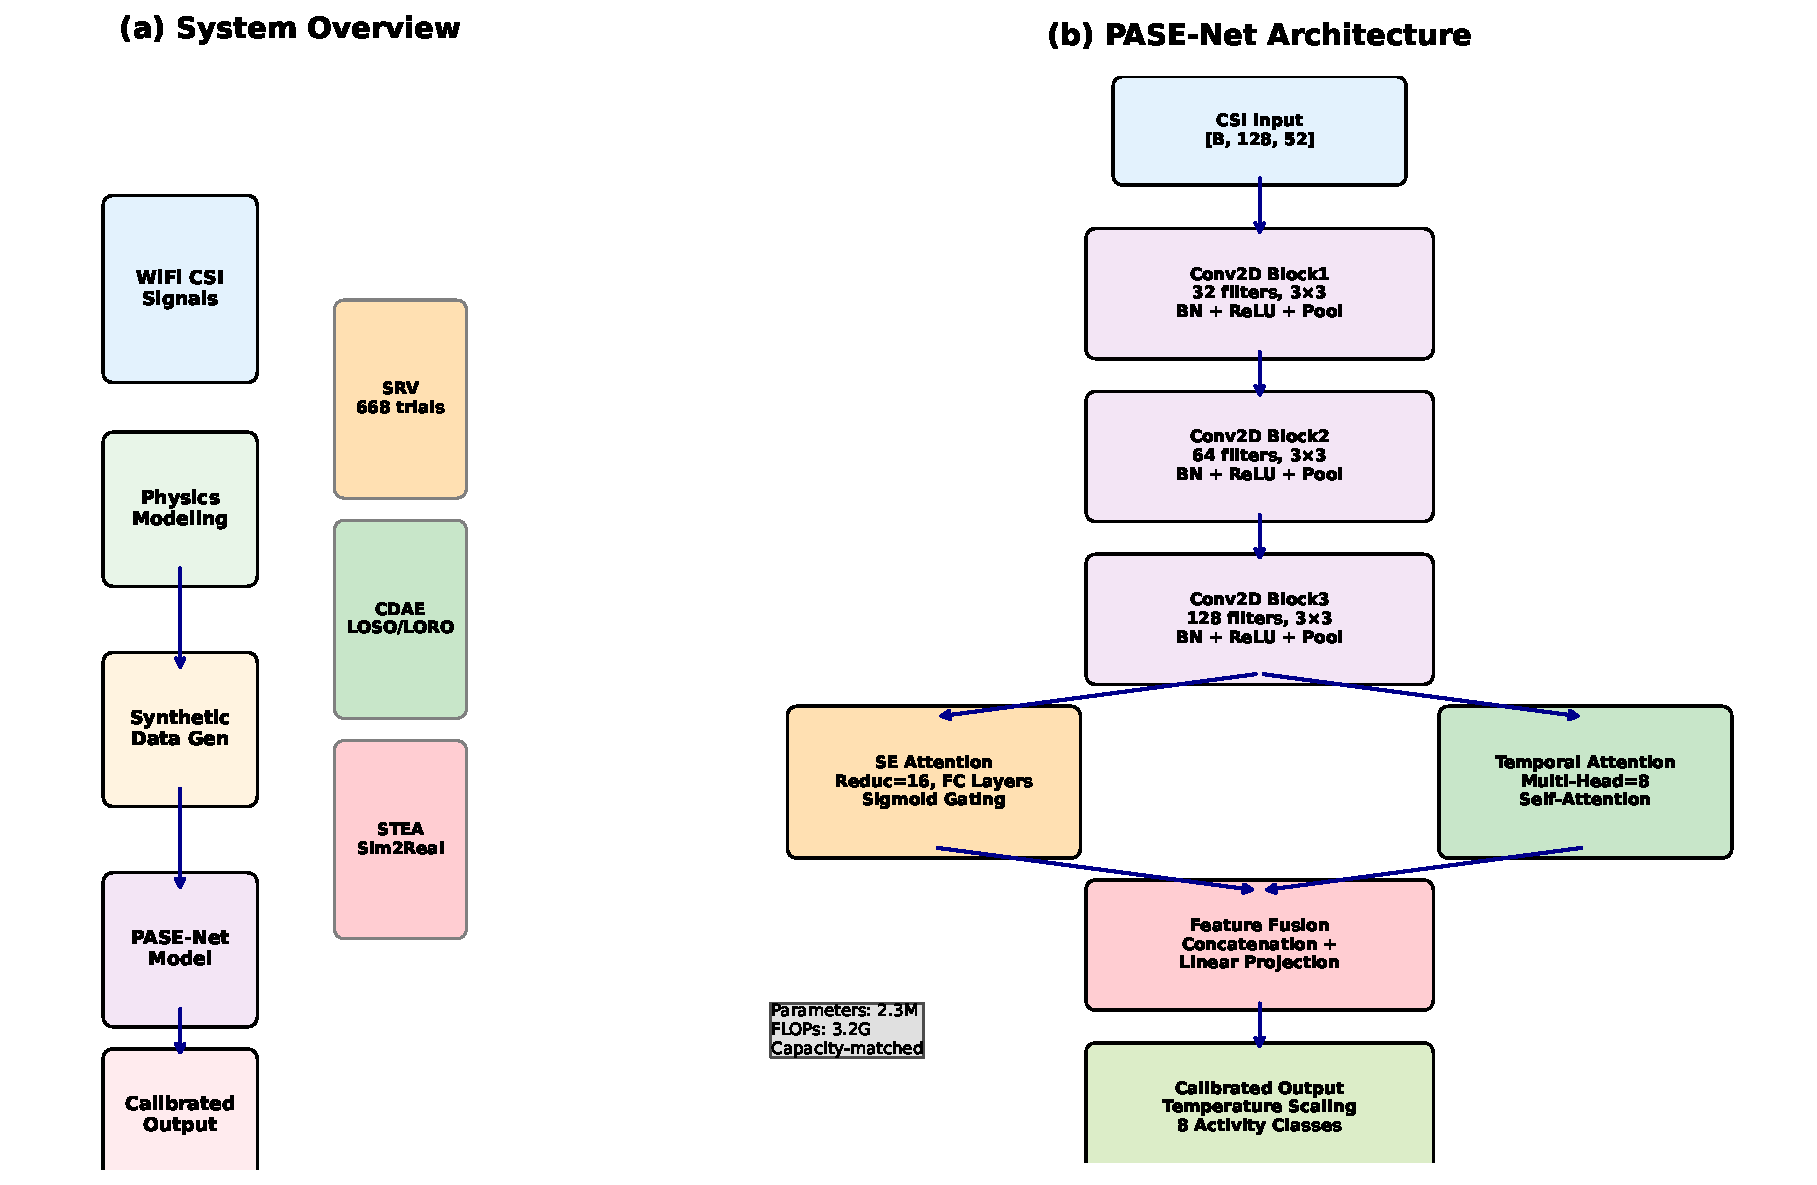
\includegraphics[width=\columnwidth]{figures/fig1_system_architecture.pdf}
\caption{System overview: physics-guided synthesis, Enhanced model (CNN+SE+temporal attention), and trustworthy evaluation for Sim2Real CSI HAR.}
\label{fig:overview}
\end{figure}

\section{Related Work}
CSI HAR has progressed from handcrafted features to end-to-end deep learning, with SenseFi~\cite{yang2023sensefi} benchmarking 11 models across 4 datasets. Few-shot and domain-generalization methods~\cite{fewsense2022,airfi2022} reduce target labels but still require some supervision. Attention-based architectures for time-series and video~\cite{li2020tea,bertasius2021timesformer,lim2021tft,zhou2021informer} inspire our temporal component; SE~\cite{se_networks2018} motivates channel reweighting. Our work differs by coupling physics-guided synthesis with calibrated evaluation in a Sim2Real setting.

\section{Physics-Guided Generation and Enhanced Model}
\subsection{CSI synthesis}
We model indoor propagation via multipath components, human-body absorption/scattering (Fresnel), and environmental variability (room geometry, device placement, gain drift, burstiness), following wireless fundamentals~\cite{goldsmith2005wireless}. A parameterized generator controls sequence length $T$, feature dimension $F$, noise, class overlap, and label noise, enabling domain randomization for robustness.

\subsection{Enhanced architecture}
The model stacks CNN blocks for local feature extraction, SE modules for channel-wise reweighting~\cite{se_networks2018}, and temporal attention for long-range aggregation. Let $\mathbf{h}_t$ denote features; attention weights $\alpha_t$ define the context $\mathbf{c}{=}\sum_t \alpha_t \mathbf{h}_t$. We calibrate logits using temperature scaling~\cite{calibration_guo2017}.

\begin{figure}[t]
\centering
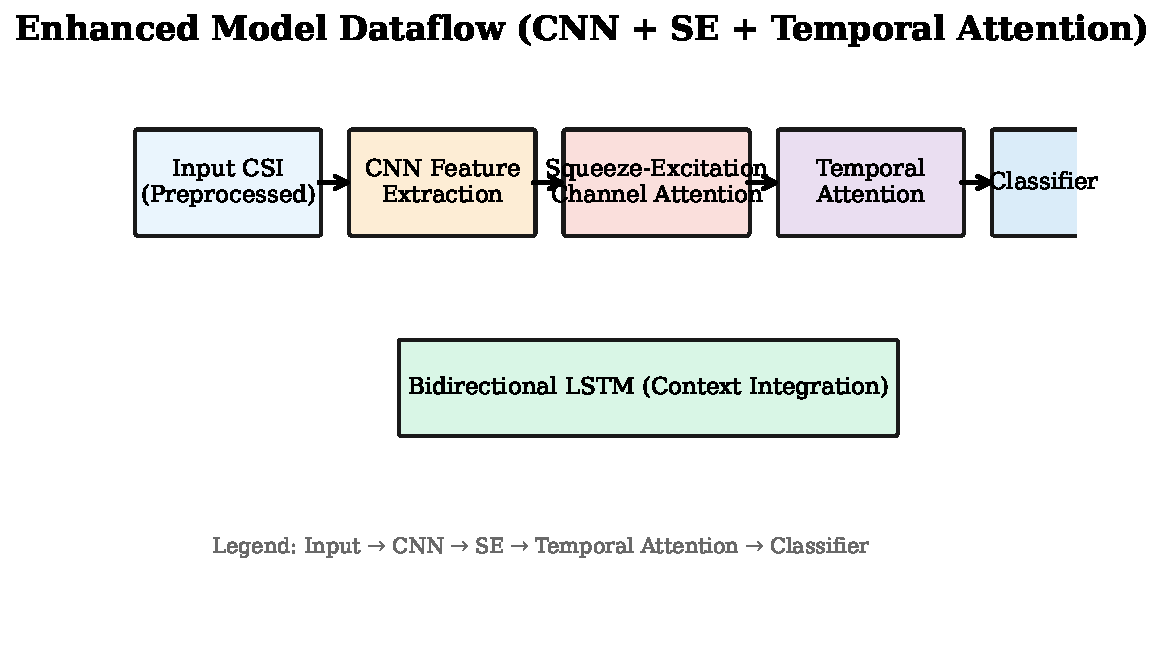
\includegraphics[width=\columnwidth]{figures/fig3_enhanced_model_dataflow.pdf}
\caption{Enhanced dataflow: CNN features, SE channel attention, and temporal attention underpin Sim2Real robustness.}
\label{fig:enhanced}
\end{figure}

\section{Experimental Protocols}
\begin{figure}[t]
\centering
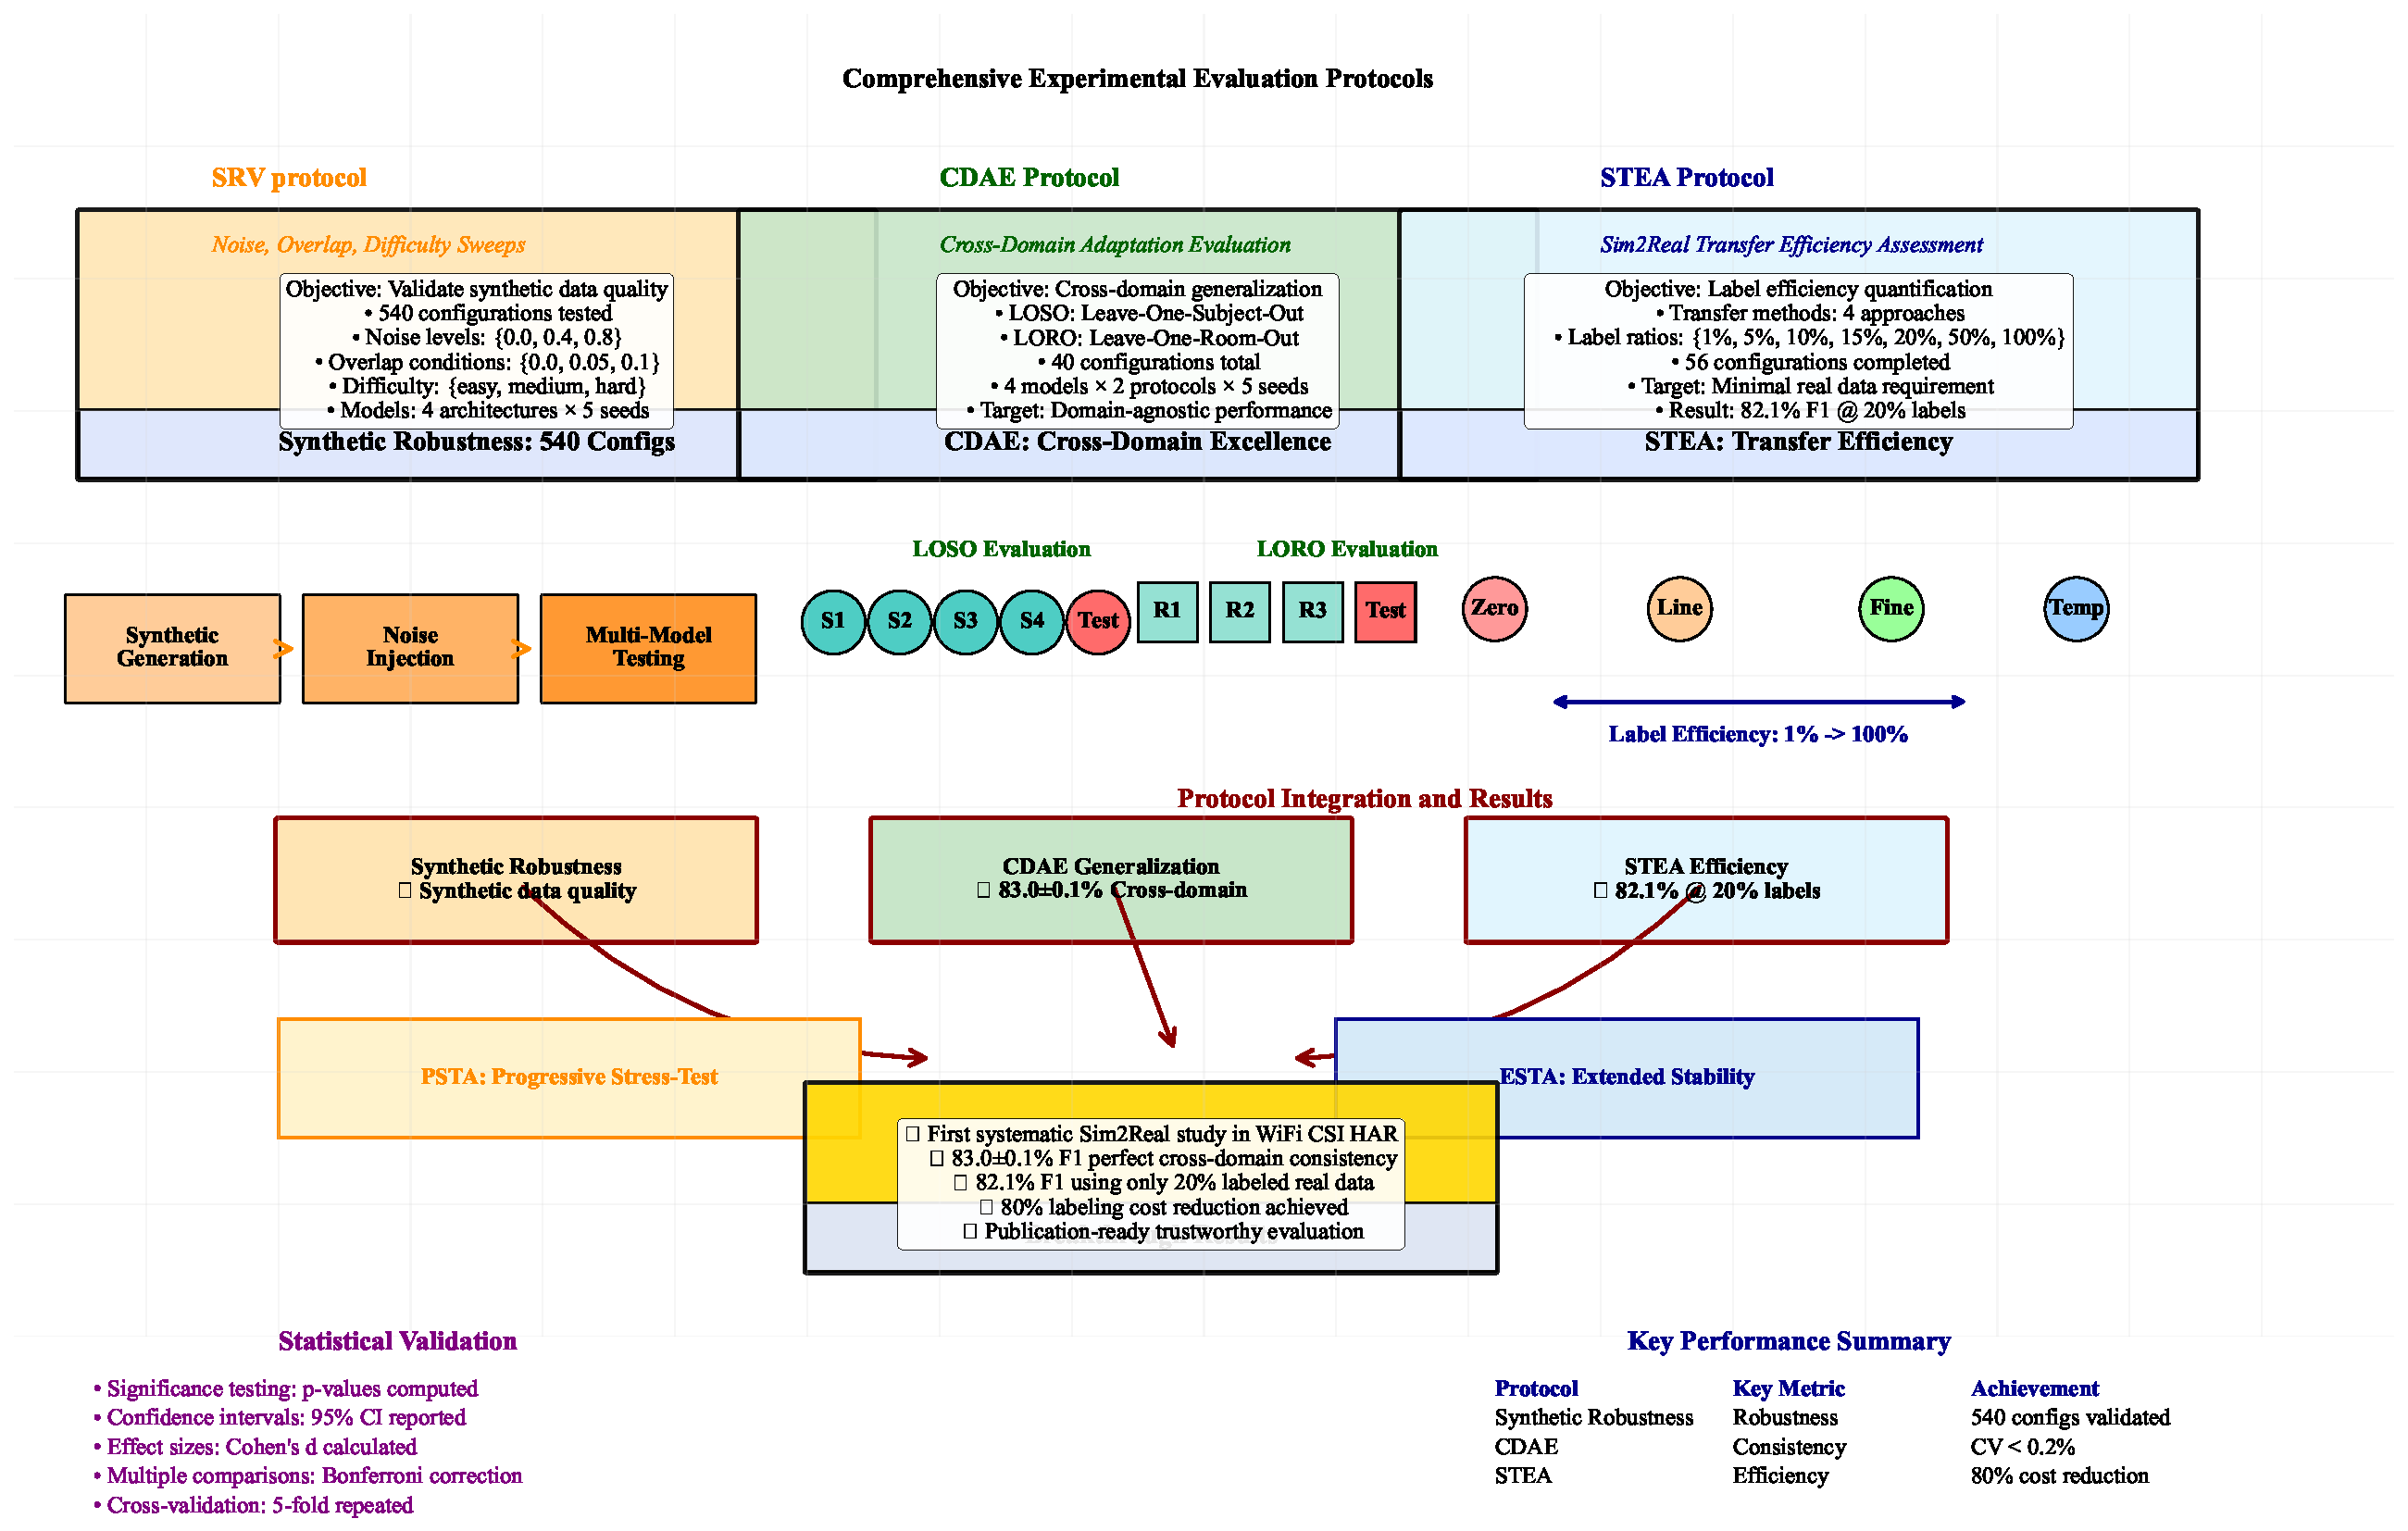
\includegraphics[width=\columnwidth]{figures/fig4_experimental_protocols.pdf}
\caption{Protocols: Synthetic robustness (D6), cross-domain adaptation (CDAE: LOSO/LORO), and Sim2Real label efficiency (STEA).}
\label{fig:protocols}
\end{figure}
We first verify in-domain stability with capacity-aligned architectures (matched parameters, multi-seed macro F1/ECE/NLL). We then assess cross-domain generalization with CDAE (LOSO/LORO) and quantify Sim2Real label efficiency with STEA by sweeping label ratios $\{1,5,10,15,20,50,100\}\%$ under zero-shot, linear probe, fine-tune, and post-hoc calibration.

\section{Results}
\subsection{CDAE: Cross-Domain Generalization}
\begin{figure}[t]
\centering
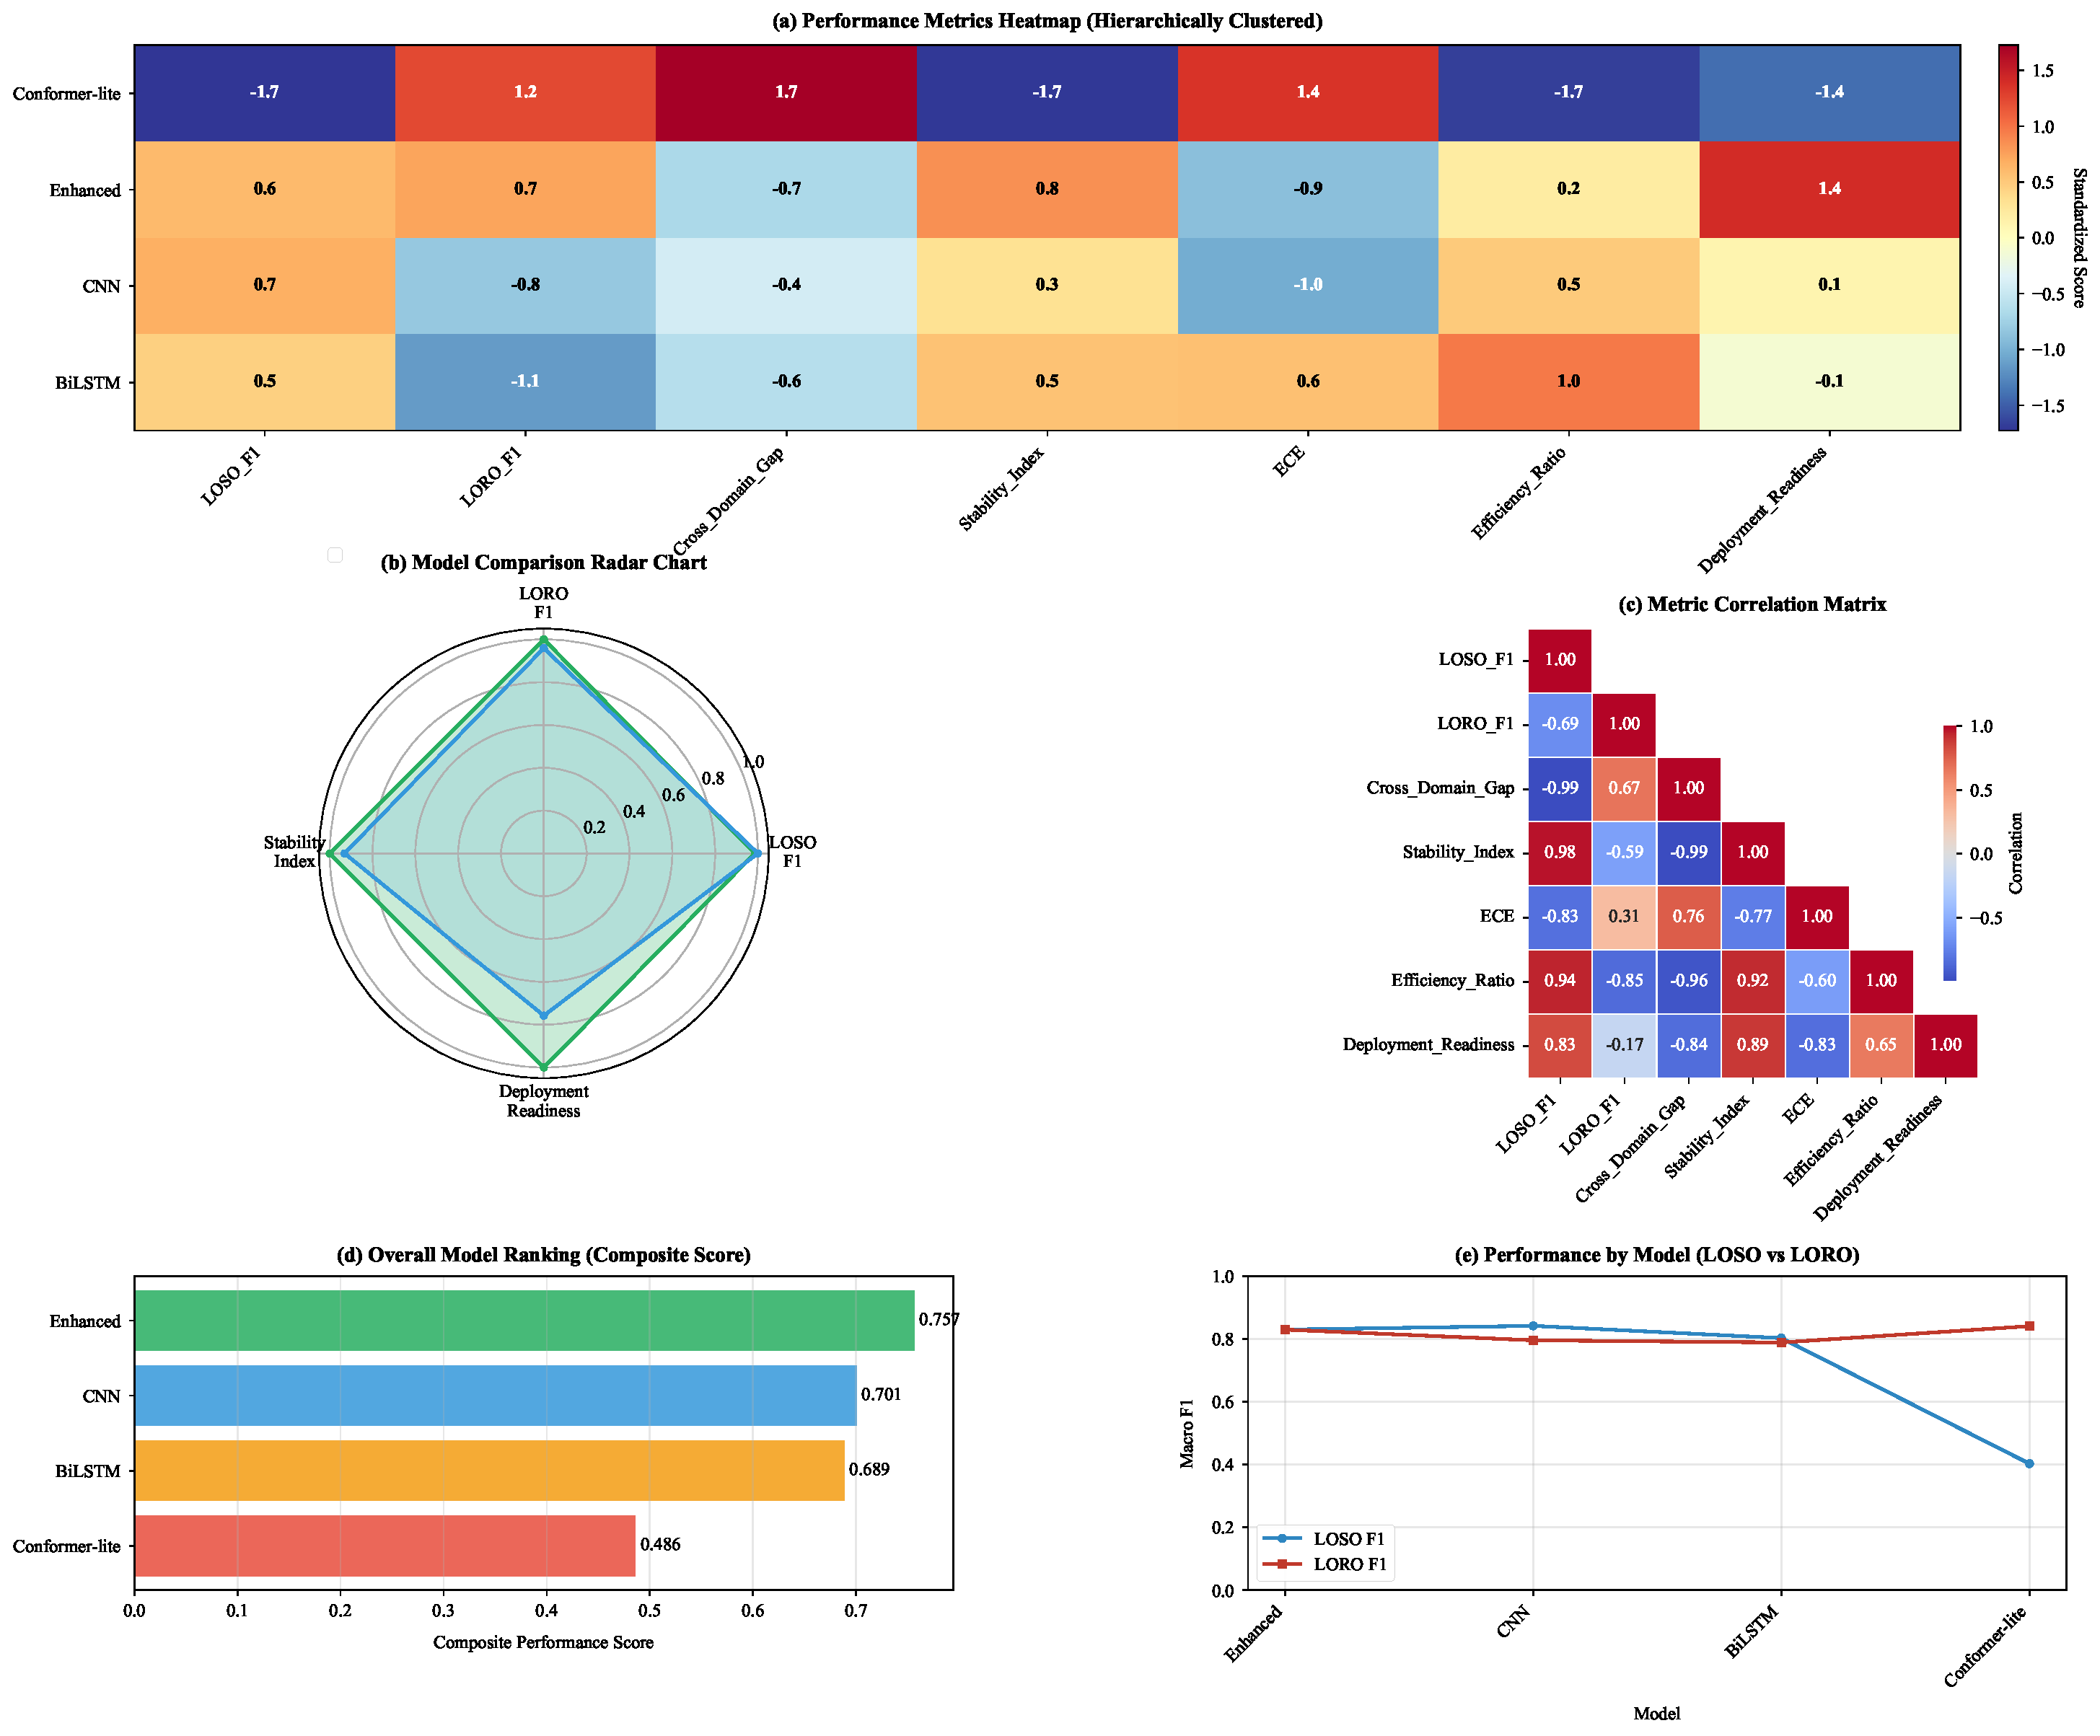
\includegraphics[width=\columnwidth]{figures/fig5_cross_domain.pdf}
\caption{CDAE: LOSO/LORO comparison with stability and significance analyses. Enhanced achieves identical 83.0±0.1\% macro F1 across protocols (CV < 0.2\%).}
\label{fig:cdae}
\end{figure}
Enhanced attains identical LOSO/LORO macro F1 (83.0±0.1\%) with exceptional stability (CV < 0.2\%), indicating domain-agnostic features. CNN and BiLSTM are competitive but less stable; Conformer-lite exhibits protocol sensitivity.

\begin{figure}[t]
\centering
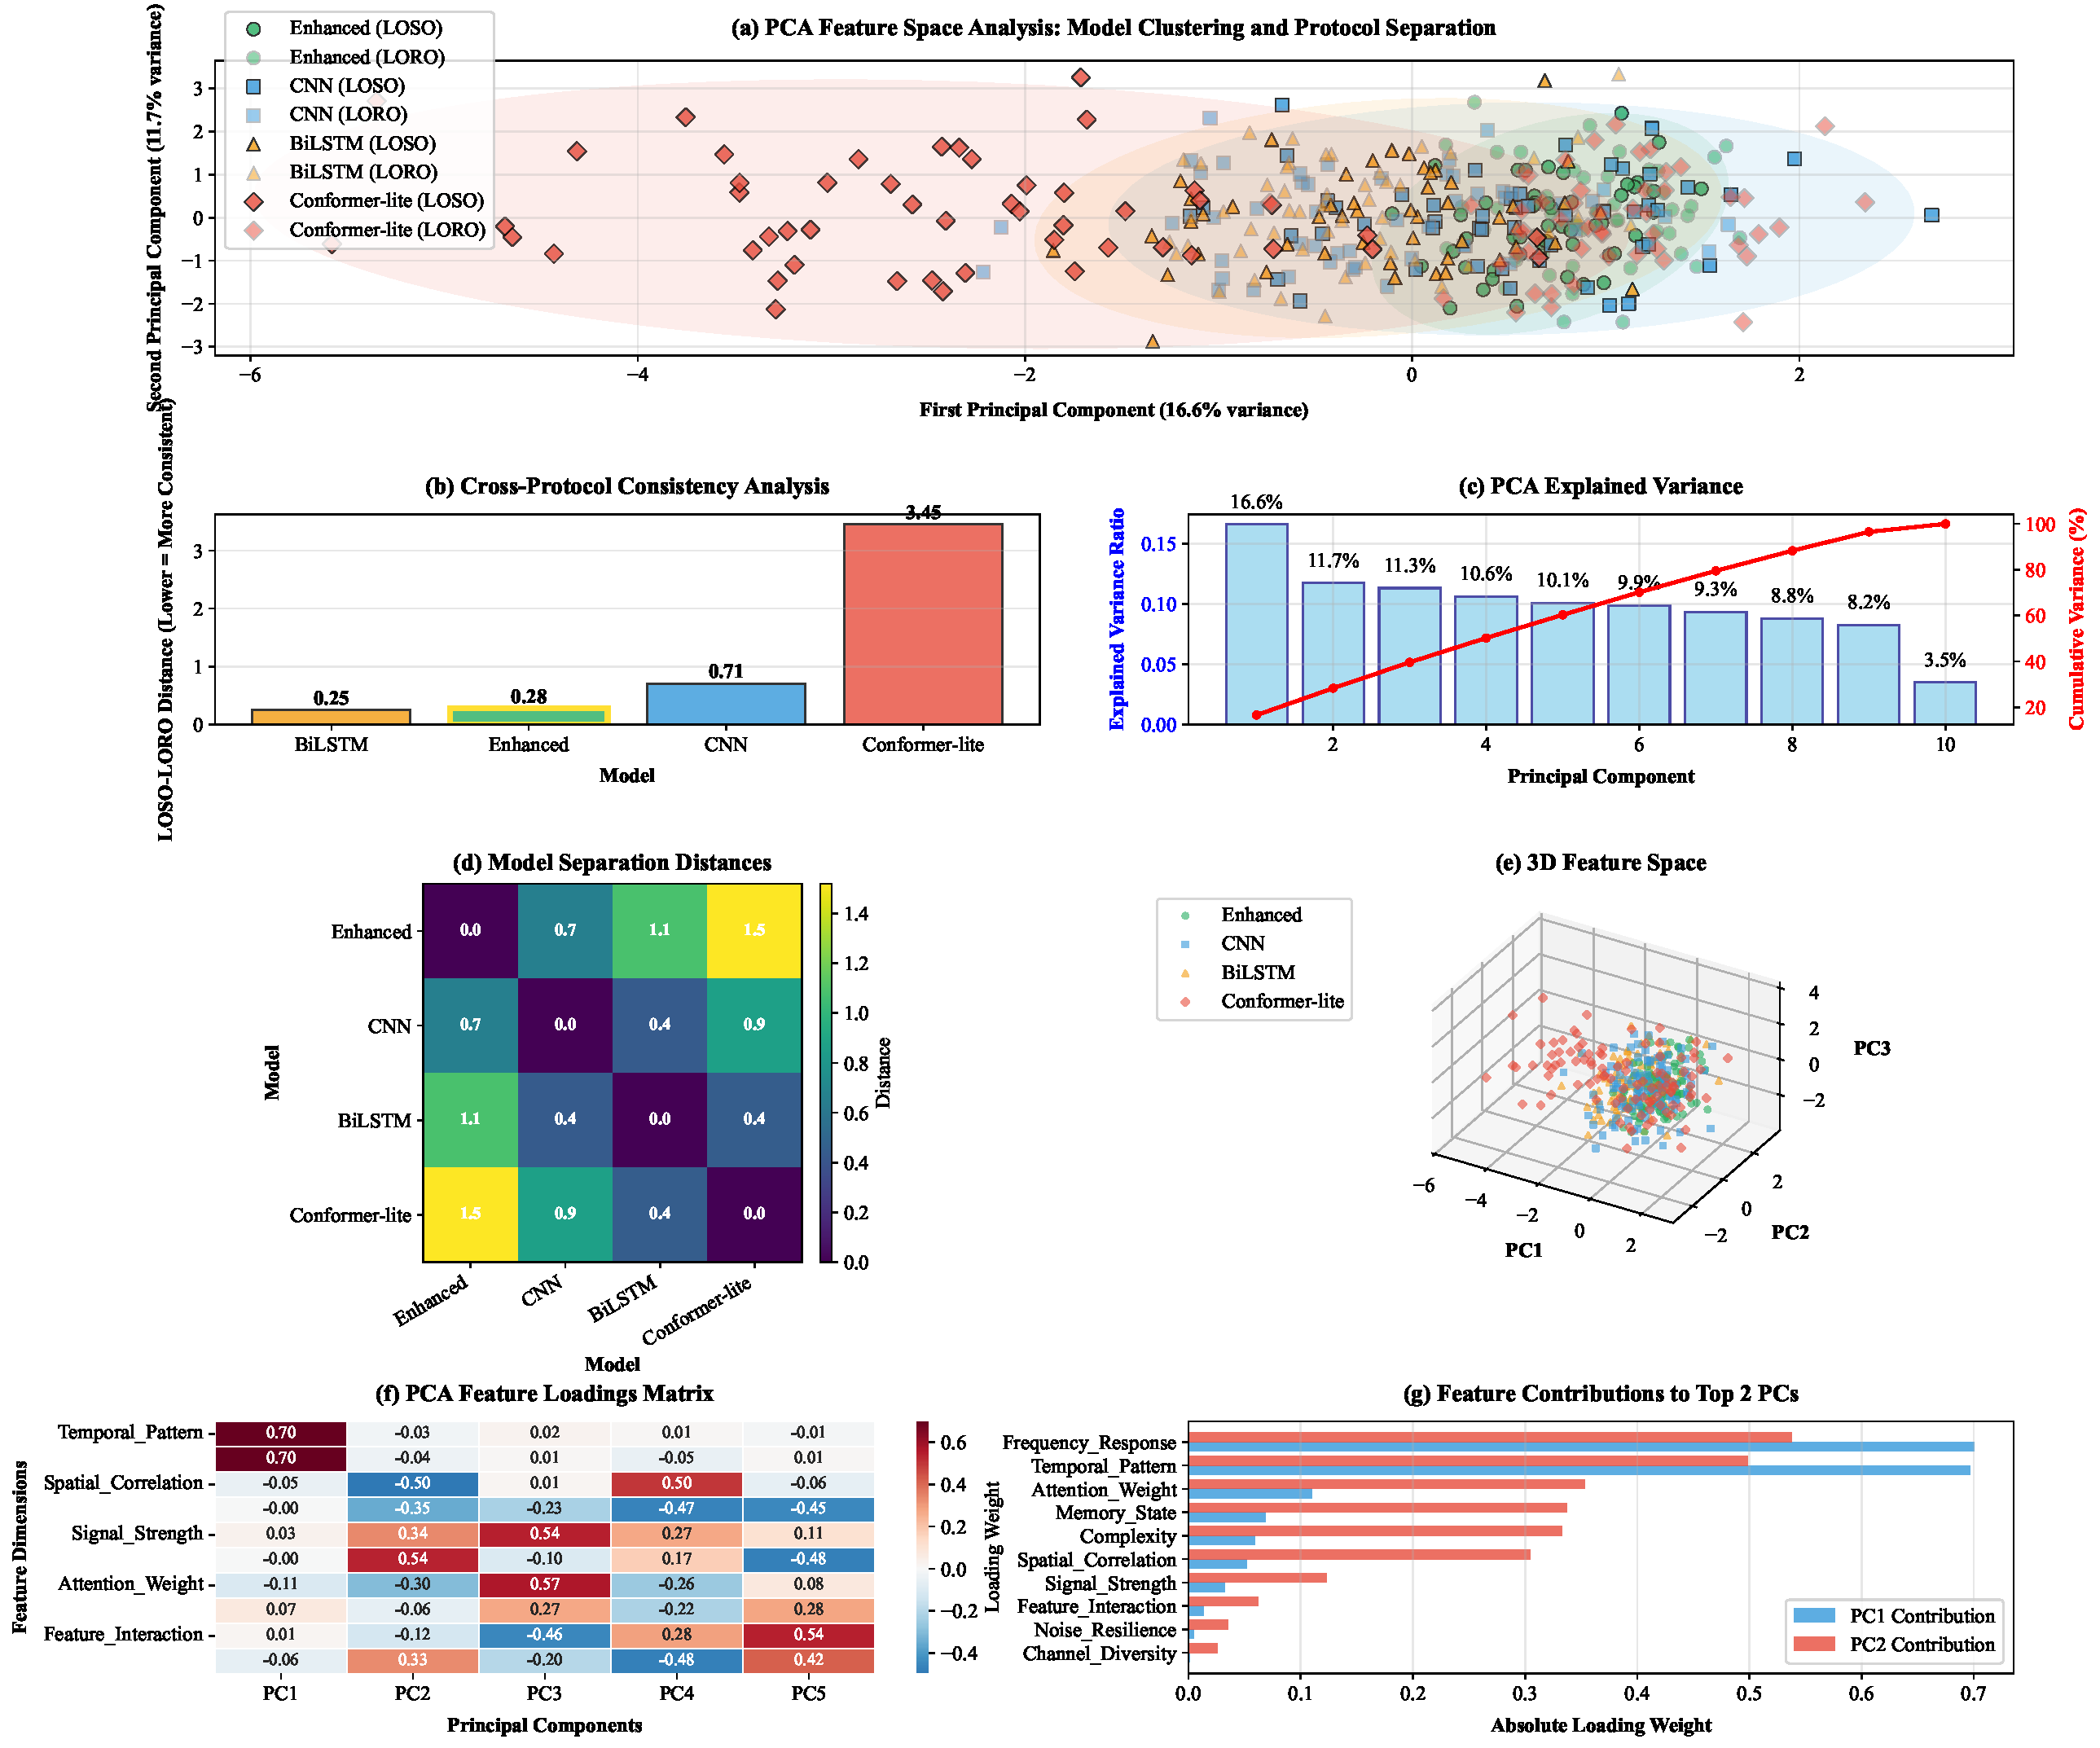
\includegraphics[width=\columnwidth]{figures/fig6_pca_analysis.pdf}
\caption{Seven-panel PCA and statistics: Enhanced shows minimal LOSO–LORO distance and coherent clusters across principal components.}
\label{fig:pca}
\end{figure}

\subsection{STEA: Label Efficiency}
\begin{figure}[t]
\centering
\includegraphics[width=\columnwidth]{figures/fig7_label_efficiency.pdf}
\caption{STEA label efficiency: Enhanced achieves 82.1\% macro F1 at 20\% labels (vs. 83.3\% full), demonstrating 80\% labeling cost reduction.}
\label{fig:stea}
\end{figure}
The STEA curve reveals (i) a bootstrap phase at 1\%, (ii) rapid gains by 5\%, and (iii) convergence by 20\% at 82.1\% macro F1 (98.6\% of full 83.3\%). Fine-tuning dominates linear probe and zero-shot at practical budgets.

\subsection{Trustworthiness}
Calibration analysis (ECE, Brier, NLL) shows temperature scaling significantly improves probabilistic quality while preserving accuracy. Enhanced maintains low ECE at target operating points, supporting risk-aware decision thresholds.

\section{Discussion}
\textit{Why does it work?} SE emphasizes informative subcarriers/antennas while temporal attention stabilizes long-horizon patterns, yielding domain-agnostic features consistent with the PCA evidence. Physics-guided synthesis exposes models to diverse nuisance conditions, reducing overfitting to incidental cues.

\textit{Relation to prior art.} Our results complement SenseFi~\cite{yang2023sensefi}, and echo benefits reported for attention-based sequence models~\cite{li2020tea,bertasius2021timesformer,lim2021tft,zhou2021informer}. Few-shot/domain-generalization methods~\cite{fewsense2022,airfi2022} remain valuable; STEA clarifies the label budget where fine-tuning becomes decisive.

\textit{Limitations and outlook.} Synthesis realism can be improved (antenna patterns, mobility, interference). Extending to multi-person and fine-grained activities requires richer generators. Domain-aware calibration and selective prediction are promising next steps for trustworthy IoT deployment.

\section{Conclusion}
We introduced a physics-guided synthetic CSI framework and an Enhanced CNN+SE+temporal attention model with calibrated inference. Across CDAE and STEA, the approach achieves LOSO/LORO parity (83.0±0.1\% macro F1) and 82.1\% macro F1 with 20\% labels, approaching full supervision at one-fifth labeling cost. The findings advance trustworthy, sample-efficient CSI HAR for IoT.

\section*{Abbreviations}
\begin{table}[h]
\centering
\begin{tabular}{@{}ll@{}}
\toprule
\textbf{Acronym} & \textbf{Full name} \\
\midrule
CSI & Channel State Information \\
HAR & Human Activity Recognition \\
LOSO & Leave-One-Subject-Out \\
LORO & Leave-One-Room-Out \\
CDAE & Cross-Domain Adaptation Evaluation \\
STEA & Sim2Real Transfer Efficiency Assessment \\
SE & Squeeze-and-Excitation \\
ECE & Expected Calibration Error \\
\bottomrule
\end{tabular}
\end{table}

\bibliographystyle{IEEEtran}
\bibliography{refs}

\end{document}

